\section{Background} \label{background}
\subsection{Instantaneous linear mixture model} \label{bssmodel}
Based on the cocktail party problem introduced in Chapter \ref{intro}, here we extent the idea of blind source separation to a formal mathematical definition. %Before that, we simply the BSS problem by applying the instantaneously linear mixture model.
The mixing process of the sources in BSS involves many models such as the instantaneous linear mixture model, the nonlinear mixture model and the convolved mixture model \cite{Hxu2014}. The instantaneous linear model omits the time delay of source propagation of reaching different observers. We assume that the instantaneous linear BSS model is adopted throughout this report.\\

\begin{figure}[H]
\centering
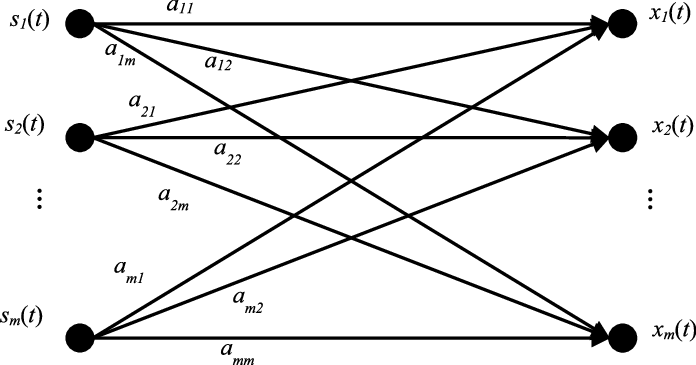
\includegraphics[width=0.45\textwidth]{images/Instantaneous-linear-mixture-model.png}
\caption{Instantaneous linear mixture model (m=n)}
\label{Ins_LMM}
\end{figure}


The instantaneously linear mixture model states that given $m$ observations $\{x_1,\cdots, x_m\}$ where each $\{x_i\}_{i=1, \cdots,m}$ is a row vector of size $t$. Each observation is the linear mixture of $n$ sources $\{s_1^T,\cdots, s_n^T\}$ weighted by $a_{ij}$

\begin{equation}
    \forall i \in \{1, \cdots, m\}, \quad x_i = \sum_{j=1}^n a_{ij}s_j
    \label{sumofs_t}
\end{equation}
Figure (\ref{Ins_LMM}) illustrates the case when we have equal number of sources and observations. Since results are not affected by reciprocal rescaling of $a_{ij}$ and $s_j$. Without loss of generality, the $a_{ij}$ will hitherto assumed to be normalised to unit length. The mixing model can be conveniently rewritten in matrix form
\begin{equation}
    \mathbf{X} = \mathbf{AS} +\mathbf{N}   
    \label{mixing}
\end{equation}

where $\mathbf{X}$ is the observation matrix with dimension $m \times t$, $\mathbf{S}$ is the $n\times t$ source matrix and $\mathbf{A}$ is the $m \times n$ mixing matrix. An $m \times t$ matrix $\mathbf{N}$ accounts for additive noise or model imperfections. Under the blind separation problem setting, both $\mathbf{A}$ and $\mathbf{S}$ are unknown.  %$\mathbf{A}$ will be assumed to be full rank when ICA is in use. 
Source separation techniques aim at recovering the original signal $\mathbf{S} = [s_1^T,\cdots, s_n^T]$ from $m$ different mixtures by taking advantage of some information in the way the signals are mixed in observed data. In other words, source separation simply boils down to devising quantitative measures of diversity or contrast to differentiate between the sources.\\

Mathematically, We aim to find a demixing matrix $\mathbf{W}$ with dimension $n \times m$ which gives a linear combination of columns in the  observation $\mathbf{X}$, omitting the noise for now, that is
\begin{equation}
    \mathbf{Y} = \mathbf{WX}
    \label{demixing}
\end{equation}

$\mathbf{Y}$ is hence an estimation of source $\mathbf{S}$.
Combining Eq. (\ref{mixing}) and (\ref{demixing}) $y$ can be written as
\begin{equation}
    \mathbf{Y} = \mathbf{W^T} \mathbf{X} = \mathbf{W A S} = \mathbf{Z^T S}
    \label{estimationYandZ}
\end{equation}
Where $\mathbf{Z^T} = \mathbf{W A}$. The estimation matrix $\mathbf{Y}$ can also be represented as 
\begin{equation}
    \mathbf{Y} = \mathbf{PDS} 
    \label{permutEQ}
\end{equation}
where $\mathbf{D}$ is a diagonal matrix and $\mathbf{P}$ is a permutation matrix that reduces the scale permutation indeterminacy of the mixing model.

\subsection{Ambiguities of BSS process}
\label{ambiguitiesBSS}
Because lack of prior knowledge about the sources and mixing process. While estimating the mixing and source matrices, we introduce the diagonal matrix $\mathbf{D}$ and permutation matrix $\mathbf{P}$ in Equation (\ref{permutEQ}), which accounts for the two ambiguities below.\\

Variances (energies) of each source component is unknown. The reason is that, both $\mathbf{S}$ and $\mathbf{A}$ are not defined, any scalar multiplication in one of the sources $s_i$ would always be cancelled by dividing the corresponding column $a_i$ by the same quantity. However, the information of sources is stored in the signal waveform rather than amplitude. This ambiguity is hence insignificant in most applications \cite{HYVARINEN2000411}. As mentioned in the last section, the columns of $\mathbf{A}$ is normalised to unity just for convenience in calculation.\\

Apart from amplitude uncertainty, we cannot determine the order of the sources. In Equation (\ref{sumofs_t}), we can freely rearrange the sources up to any permutation without affecting the observation samples. Any of the source components can be regarded as the first one. Again, Because the information of each component is contained in the shape of waveform of that component, not the order of components. So this ambiguity is also insignificant.



\subsection{Preprocessing of BSS techniques}
Before applying the BSS methods on the data, it is usually very usful to do some preprocessing. In this section, we introduce two preprocessing techniques that make the blind source separation problem simpler and better conditioned.
Centering:
Most BSS methods assumes the data to be zero centered. The most basic and necessary preprocessing is to center the observation data $x_i$ by substract the sample mean from it. 
Whitening:
Before applying BSS methods (and after centering), the observed vector $x$ is linearly transformed to $\tilde{x}$ so that each column is uncorrelated and have unity variance. More specifically, the covariance matrix of $\tilde{x}$ equals the identity martix, $\E\{\tilde{x}\tilde{x}^T\} = \mathbf{I}$. The most common used whitening transformation is eigenvalues decompostion (EVD) of the data covariance matrix.

\subsection{BSS Performance Measures}
\label{perform_metric}

\subsubsection{Correlation coefficient}
Correlation coefficient measures the similarity between a recovered source $S^{'}$ and the original source $S$.
\begin{equation}
    \rho = \frac{\text{cov}(S^{'},S)}{\sigma_x \sigma_y}
\end{equation}

\subsubsection{Mixing matrix criterion}
Mixing Matrix Criterion assesses the separation quality due to demixing matrix $\mathbf{A}$, especially in noisy content.
\begin{equation}
    C_A = ||\mathbf{I_n} - P\tilde{\mathbf{A}}^{+}\mathbf{A} ||
\end{equation}

where $\mathbf{I}$ is the identity matrix, $\mathbf{P}$ is the permutation matrix, and $\tilde{\mathbf{A}}^{+}$ is the pseudo-inverse of the estimated mixing matrix. The mixing matrix criterion is strictly positive, unless the mixing matrix is correctly estimated up to scale and permutation \cite{VAbolghasemi2012}. Low values of $C_A$ then indicate better separation performance.
 
\subsubsection{Human visual system (HVS)}
Most of out work in this report focus on blind image separation. Human visual system says that people are not as sensitive to high frequency detail as to low frequency ones. Therefore, standard metrics may not best describe the actual experiment outcomes. In order to better evaluate the results in image processing, we adopt HVS as the subjective metric.

\subsection{Applications of BSS}
The classical application of BSS on the cocktail party problem is trying to understand how the humans select the voice of a particular speaker from an ensemble of different voices corrupted by music and noise in the background. Other applications, besides the cocktail party problem mentioned in the introduction, have also attracted researchers' attention in the past decade. Examples are given as below. \\

An electroencephalogram (EEG) is a test used to find problems related to electrical activity of the brain. In EEG analysis, different artifacts such as eye-blinking deteriorate its quality. Identification of the various sources from the independent components is thus integral for clinical analysis. An innovative method combining the use of standard BSS techniques and Support Vector Machines (SVM) was applied to solve this problem  \cite{Duda2000PC954544}.\\

Filling `holes' in images is an interested and important inverse problem with applications in repairing the old and deteriorated artwork. Based on Morphological Component Analysis, an inpainting algorithm has been proposed  which is capable of filling holes in either texture or cartoon content \cite{ELAD2005340}. The inpainting algorithm is applied on the famous Barbara images and achieve satisfactory result even when there are 80\% missing pixels. \\

\begin{figure}[!htbp]
\centering
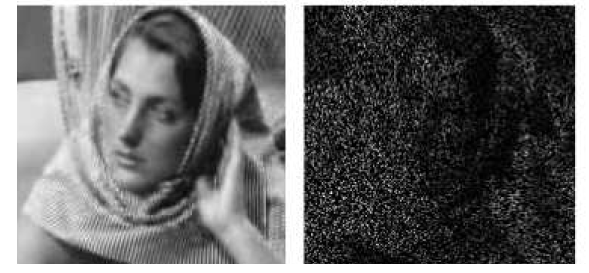
\includegraphics[width=0.45\textwidth]{images/impainting1.png}
\caption{Barbara image with $80\%$ missing pixels (right). The result of the MCA impainting is
given on the left.}
\label{imapint1}
\end{figure}

In Code-Division Multiple Access (CDMA), blind separation techniques are used to suppress unintentional multiuser interference (jammer), separate the desired user signals from other users' signals \cite{Raju2006}. BSS also has wide applications in military based telecomm systems which recovers radar reflection from strong intentional interference.\\

BSS is also closely related with studying the underlying factors of the financial data and driving mechanisms behind financial time series. In \cite{OjaE2000Icaf} ICA is applied to financial time series data. The data is parallel, representing the simultaneous cash flow at several stores belonging to the same retail chain. The ICA finds the fundamental factors that are common to all stores that affect the cashflow data, although each store responds to these factors in a slightly different manner. Thus, the cashflow effect of the factors specific to any particular store could be revealed.

\subsection{Independent Component Analysis}
ICA algorithms are about devising appropriate independence approximations. This includes, maximisation of non-Gaussianity, minimisation of mutual information and maximum likelihood estimation \cite{HYVARINEN2000411}. ICA based neural network \cite{Bell1995AnIA} was also proposed based on maiximing the output entropy of a neural network with non-linear outputs. We are not going to discuss these approximations in depth as we want to focus more on the sparsity based blind source separation. However, FastICA and JADE are introduced below.\\

FastICA calculates the negentropy as an approximate of independence measure. With a taste of the Central Limit Theorem, intuition tells us that the distribution of a sum of independent random variables tends to toward a Gaussian distribution, under certain conditions. Known from Equation (\ref{estimationYandZ}) that $y = w^T x = w A s = z^T s$. It is clear that the closest estimation is when $z^Ts = s$ which also has the least Gaussianity. Hence finding independent $s$ is equivalent to minimisation of Gaussianity. The approximation of non-Gaussianity is based on a maximum negentropy principle.
\begin{equation}
    J(y) \propto [E\{G(y)\} - E\{G(v)\}]^2
\end{equation}
Where $v$ is a standardised Guassian variable. And $G$ are predefined functions with the possible choices stated in \cite{HYVARINEN2000411}. In general, FastICA is based on a fixed point iteration scheme for finding the maximum of non-Gaussianity of $\mathbf{w^T x}$ in Equation (\ref{demixing}). The basic form of FastICA algorithm is as follows.

% -------------------- algorithm block ------------------------
\begin{algorithm}[!htbp] 
\caption{ The basic FastICA algorithm for estimating one independent component}
\label{alg:Framwork} 
\begin{algorithmic}
\REQUIRE ~~\\%Input
The observed matrix $\mathbf{x}$
\ENSURE ~~\\ %Output
Estimation of $\hat{\mathbf{A}}$
\STATE 1. Choose an initial (e.g. random) wright vector $\mathbf{w}$
\STATE 2. Let $\mathbf{w}^+ = E\{\mathbf{x}g(w^T x) - E(g'(w^Tx)\}\mathbf{w})$
\STATE 3. Calculate $\mathbf{w} = \mathbf{w}^{+}/\lVert w^{+}\rVert$
\STATE 4. If not converged (old and new values of $\mathbf{w}$ point in the same direction up to multiplicative signs), return to step 2
\end{algorithmic}
\end{algorithm}
% -------------------- algorithm block ------------------------

JADE is based on similar ideas of the FastICA agorithm apart from it calculates the fourth-order statistics (Kurtosis). JADE finds out the direction where the kurtosis of observed signal grows most strongly (super-Gaussian signals) or decreases most strongly (sub-Gaussian signals).\\

\label{ica_defect}
ICA suffers from several limitations which make it unsuitable in some specific applications. Firstly, ICA require the mixing matrix $\mathbf{A}$ to be full rank and square. As we mentioned in the introdcution, generally ICA cannot be applied to the underdetermined mixing scenario. Secondly, ICA also assumes that amongst the components in $\mathbf{s}$, there exists at most one component that is Gaussian. This means ICA is not robust under the additive Gaussian nosie setting. While even implicit, the ICA algorithm requires information on the source distribution when doing separating computation such as maximum likelihood estimation, making it hard for model generalisation. We will exam the limitations of ICA in future simulations.

\subsection{Sparse representations of signals}
Here we introduces the idea of sparse signal processing and how it helps to solve underdetermined linear systems (dictionary). However we need to discriminate the expression from the underdetermined system mentioned in previous parts. In BSS, `underdetermined system' means linear combination of \textbf{source signals} while here we refer to further linearly decompose the source signals into a given \textbf{dictionary}. In a more plain language, less number of examples than the data dimensionality involved are available for learning the dictionary. Sparse signal processing has numerous applications in compress sensing, image deniosing and super-resulation reconstrcution.

\subsubsection{Overcomplete dictionary}
\label{over_dict}
The key idea of sparse signal representation is to assume
that the sources are sparse, or can be decomposed into the
combination of a small number of signal components. By
sparse, we mean that most values in the signal or its transformed coefficients are zero. These signal components are called atoms, and the collection of all the atoms is referred to as a dictionary \cite{Mallat_Zhang1993}. In the general sparse representation framework, we can model a signal $y \in R^N$ as the linear combination of $D$ elementary signal atoms in dictionary $\mathbf{\Phi}$, such that.

\begin{equation}
    y = \alpha \mathbf{\Phi}
    \label{dict_qe1}
\end{equation}
where $\alpha$ is called the representation coefficients of $y$ in the dictionary $\mathbf{\Phi}$
%= \{\Phi_1, \cdots, \Phi_D \}
(the $N \times D$ matrix). 
In the case of overcomplete representations, the number of waveforms or atoms ($\varphi_i$) is higher than the dimension of the space in which $y$ lies, that is $D > N$. 

\begin{figure}[!htbp]
\centering
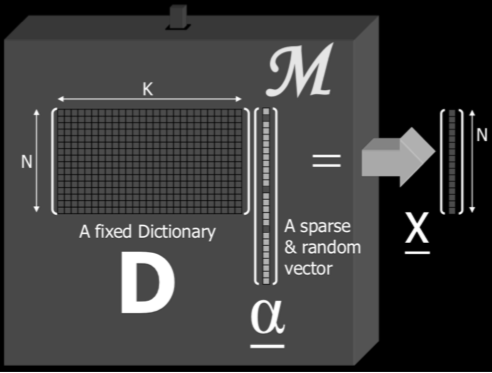
\includegraphics[width=0.45\textwidth]{images/dictionary_sparse.png}
\caption{Illustration of sparse representation using overcomplete dictionary}
\label{dic1}
\end{figure}

\subsubsection{Sparse decomposition}
\label{BSS_sparse_decomp}
The decomposition problem of a signal or image in predefined $\mathbf{\Phi}$ amounts to recovering the coefficient vector $\alpha$ in Equation (\ref{dict_qe1}). When $\mathbf{\Phi}$ is overcomplete, the solution is generally not unique. In that case, our goal is to recover the sparsest solution $\alpha$ which requires solving:
\begin{equation}
    \min_{\alpha}||\alpha||_0 \quad \text{s.t.} \quad y = \alpha \mathbf{\Phi}
\end{equation}

However, the above equation leads to an NP-heard optimisaation problem due to its non-convextivity. Alternatively, we convexify the constraint by substituting the convex $\ell_1$-norm with the $\ell_0$-norm, leading to the following equation:
\begin{equation}
    \min_{\alpha} ||\alpha||_1 \quad \text{s.t.} \quad y = \alpha \mathbf{\Phi} 
    \label{l1_sparse}
\end{equation}
or\\
\begin{equation}
    \min_{\alpha}||\alpha||_1 \quad \text{s.t.} \quad || y - \alpha \mathbf{\Phi}||_2 \leq \sigma
\end{equation}

Such relaxations have led to a wide range of algorithms for signal reconstruction: the \textit{Basis Pursuit} based on linear programming  \cite{BPAtomicDcomp}, the greedy algorithm such as \textit{Matching Pursuit} \cite{Mallat_Zhang1993} and subspace techniques such as \textit{Subspace Pursuit} \cite{WdaiSP} and \textit{CoSaMP} (Compressive
Sampling Matching Pursuit) \cite{CoSaMP2008}.


\subsection{Sparsity and morphological Diversity}
In this section, we provide essential insights into the use of sparsity in BSS and we highlight the central role played by morphological diversity as a way of contrast between the sources.

\subsubsection{Morphological component analysis (MCA)}
We now introduce a practical algorithm named the morphological component analysis (MCA) aiming at decomposing signals in overcomplete dictionaries composed of a union of orthonormal basis, i.e. our dictionary is a concatenation of sub-dictionaries. In MCA setting, $y$ is a linear combination of $D$ morphological components. 
\begin{equation}
    y = \sum_{i=1}^D  \alpha_i \mathbf{\Phi}_i = \sum_{i=1}^D \varphi_i
    \label{Eq_dictionary}
\end{equation}
where $\mathbf{\{\Phi}_i\}$ are orthonormal basis whose columns are the atoms and is general normalised to a unit $\ell_2$-norm. Morphological diversity then relies on the incoherence between the subd-ictionaries. In terms of $\ell_0$-norm, this morphological diversity can be formulated as follows:
\begin{equation}
    \forall\{i,j\} \in \{1,\cdots,D\};\quad j \neq i \Rightarrow \; \lVert \varphi_i \Phi_i^T \rVert_0 < \lVert \varphi_j \Phi_i^T \rVert_0
\end{equation}
Intuitively, we can always find a sub-dictionary that one morphological component is highly sparse in it whereas other components are not sparse. We therefore estimate the morphological components $\{\varphi_i\}_{i=1,\cdots,D}$ by solving the following convex minimisation problem.
\begin{equation}
    \{\varphi_i\} = \text{Arg} \: \min_{\{\varphi_i\}}\sum_{i=1}^D \lVert\varphi_i \mathbf{\Phi}_i^T \rVert_{1} + k \:\lVert y-\sum_{i=1}^D\varphi_i \rVert^2_2 +  \sum_{i=1}^D \gamma_i C_i (\varphi_i)
    \label{MCAequation}
\end{equation}
where $C_i$ implements constraints on component $\varphi_i$. Note that this minimisation problem differs from the problem setting in Equation (\ref{l1_sparse}) by relaxing the equality constraints to the later punishment term. A fast numerical solver called the \textit{Block-Coordinate Relaxation Method} \cite{BlockCoordinateMethod} was proposed to solve this kind of optimisation problem. 
The algorithm is given as follows:

\begin{algorithm}
\caption{The numerical algorithm for MCA} 
\label{algFramwork1} 
\begin{algorithmic} %这个1 表示每一行都显示数字
\REQUIRE ~~\\%Input
The sources $y$, dictionary $\Phi$, number of morphological components $D$, number of iterations $L_{max}$ and threshold $\delta$
\ENSURE ~~\\ %Output
Each morphological components $S_k$\\
\STATE Initialize $L_{max}$; number of iterations; threshold $ \delta= k L_{max}$;
\STATE 1. Perform $J$ times:
\STATE \qquad 2. Perform $D$ times:
\STATE \qquad \quad Update of $\varphi_i$ assuming all $\varphi_l$, $l \neq i$ are fixed:
\STATE \qquad \quad - Calculate the residual $r = \varphi − \sum_{l=1, l \neq i}^D \varphi_l$
\STATE \qquad \quad - Calculate the transform $\mathbf{\Phi^T}$ of $\varphi_i + r$and obtain $a_i = \mathbf{\Phi_i^T} (\varphi_i + r)$
\STATE \qquad \quad - Soft threshold the coefficient $a_i$ with the $\delta$ threshold and obtain $\Hat{a}_i$.
\STATE \qquad \quad - Reconstruct $\varphi_i$ by $\varphi_i = \mathbf{\Phi}_i \Hat{a}_i$
\STATE \qquad \quad - Apply the constraint correction $\varphi_i = \varphi_i - \mu \gamma_k \frac{\partial C_i}{\partial s_i}$
\STATE \qquad \quad - The parameter $\mu$ is chosen either by a line-search minimizing the overall 
\STATE 3. Update the threshold by $\delta = \delta - k$.
\STATE 4. If $\delta  > k$, return to Step 2. Else, finish.
\end{algorithmic}
\end{algorithm}

\subsubsection{Mutichannel morphological component analysis (MMCA)}
In this section, we extend the monochannel sparse decomposition problem described and characterized in last section to multichannel data. In the MMCA setting, we assumed that the sources $\mathbf{S}$ in Equation (\ref{mixing}) have strictly different morphologies (i.e. each source $s_i$ is assumed to be strictly sparsely represented in one particular orthonormal basis $\mathbf{\Phi}_i$) \cite{BobinJ_2007SaMD}. Figure \ref{illu_mca_and_gmca} precisely reveals the difference between MCA and MMCA. The top observation can be strictly divided in to texture and gaussian parts whereas the bottom multichannel observations are complex combinations of curvelets and texure components.\\

\begin{figure}[!htbp]
\centering
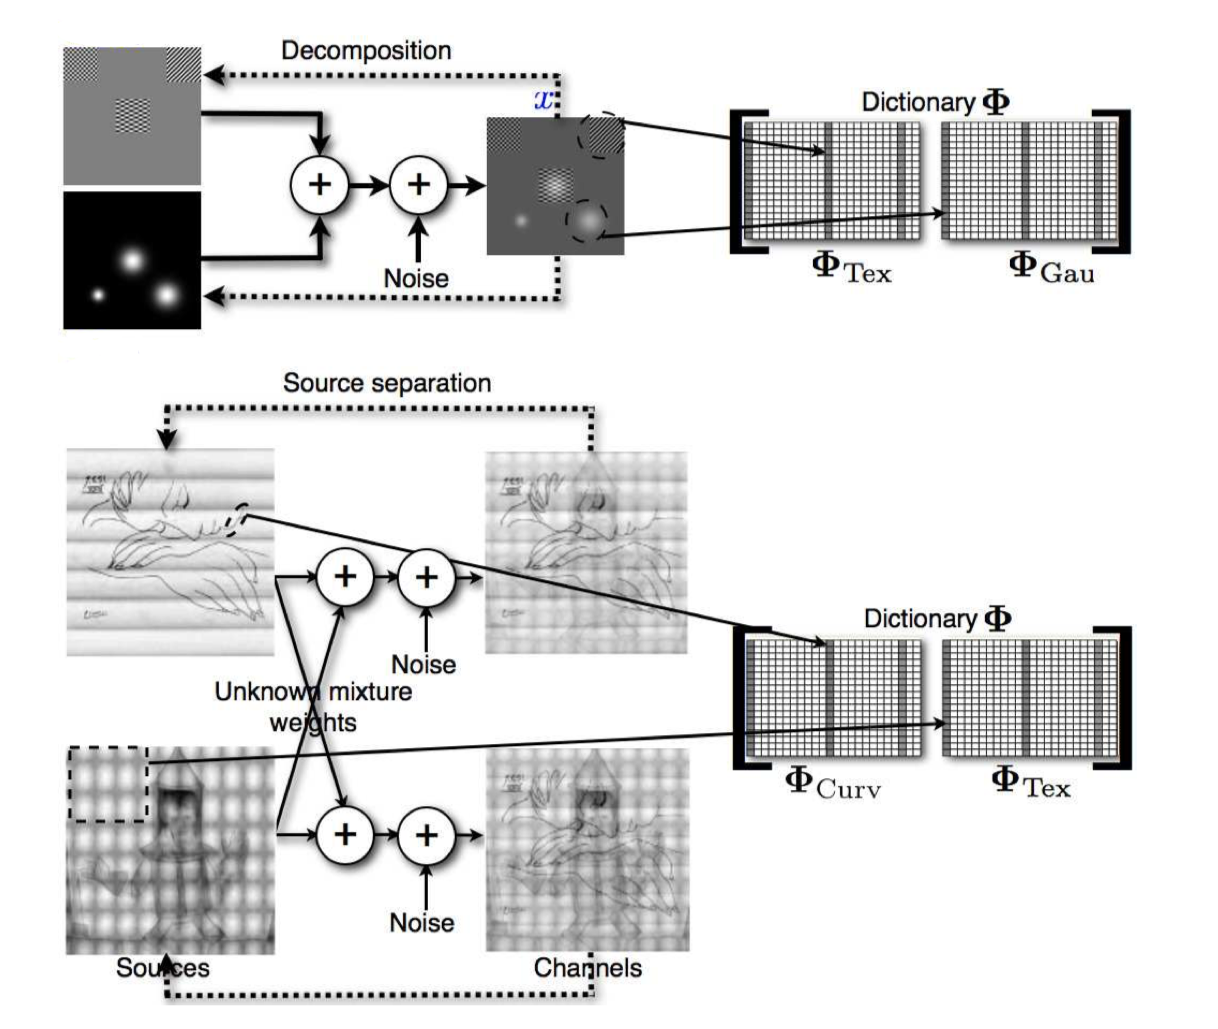
\includegraphics[width=0.7\textwidth]{images/mca_gmca.png}
\caption{Illustration of the image decomposition(top) using MCA and the blind source separation (bottom) using GMCA. For the bottom part, each source is itself a mixture of morphological components(texture and cartoon)}
\label{illu_mca_and_gmca}
\end{figure}

An iterative thresholding Block-Coordinate Relaxation algorithm similar to Algorithm (\ref{algFramwork1}) was proposed to solve the joint optimisation problem below.
\begin{equation}
    \{\mathbf{\tilde{A},\tilde{S}}\} = \text{Arg} \: \min_{\mathbf{A},\mathbf{S}}\sum_{k=1}^N \lVert s_k \mathbf{\Phi}_k^T \rVert_{1} + \lambda \:\lVert \mathbf{X} - \mathbf{AS} \rVert^2_2
    \label{MMCAequation}
\end{equation}
The equation above is very similar to Equation (\ref{MCAequation}) in MCA. Unfortunately, this MMCA criterion suffers from several drawbacks and particularly from an indeterminacy attached to the model structure \cite{BobinJ_2007SaMD}. For instance, the minimisation of this criterion may result in trivial solutions : $\mathbf{A} = \rho \mathbf{A}$ and $\mathbf{S} = \frac{1}{\rho} \mathbf{S}$ (the sparsity term can be minimised as desired as long as $\rho$ tends to $+\infty$) \cite{BobinJ_2007SaMD}. We therefore normalise the columns in matrix $\mathbf{A}$ at each iteration, as mentioned in Chapter \ref{ambiguitiesBSS}.\\

Let's introduce the $k^{\text{th}}$ channel residual $D_k = X - \sum_{j \neq k}a^j s_{j}$ (accounts for the part of that data unexplained by the other couples $\{a^j, s_j\}j \neq k$), the minimisation of the whole criterion (\ref{MMCAequation}) is equivalent to this joint minimisation problem.
\begin{equation}
    \{\tilde{s}_k, \tilde{a}^k\} = \text{Arg} \: \min_{\mathbf{A},\mathbf{S}} \lVert s_k \mathbf{\Phi}_k^T \rVert_{1} + \lambda \:\lVert D_k - a^ks_k \rVert^2_2
    \label{MMCAequation2}
\end{equation}
If we also assume the noise covariance matrix $\Gamma_n$ is known, the criterion new becomes:
\begin{equation}
    \{\mathbf{\tilde{A},\tilde{S}}\} = \text{Arg} \: \min_{\mathbf{A},\mathbf{S}} \lVert s_k \mathbf{\Phi}_k^T \rVert_{1} + Trace \{ (D_k - a^ks_k)\Gamma^{-1}(D_k - a^ks_k)^T\}
    \label{MMCAequation3}
\end{equation}
Zero the garident with respect to $s_k$ and $a^k$ leads to the following coupled equations
\begin{equation}
    \begin{cases}
       s_k = \frac{1}{a^k\Gamma^{-1}a^k}({a^k}^T - \frac{1}{2\lambda_k} Sign(s_k \mathbf{\Phi}_k) \mathbf{\Phi}_k^T)\\
       a^k = \frac{1}{s_ks_k^T}D_k s_k^T
    \end{cases}
\end{equation}
We then use the soft thresholding algorithm to solve for approximation of $s_k$ and $a_k$. Setting the threshold $\delta = \frac{\lambda_k}{2\lVert a^k\Gamma^{-1}a^k \rVert}$. Then considering a fixed $s_k$, the update on $a_k$ follows a simple least square linear regression.\\

\begin{algorithm}[!htbp] 
\caption{ The numerical algorithm for MMCA} 
\label{alg:Framwork} 
\begin{algorithmic}
\REQUIRE ~~\\%Input
The sources $S$, dictionary $\Phi$, number of morphological components $N$, number of iterations $L_{max}$ and threshold $\delta = k \cdot L_{max}$
\ENSURE ~~\\ %Output
Estimation $\hat{\mathbf{A}}$ and $\hat{\mathbf{S}}$
\STATE 1. Perform J times:
\STATE \qquad 2. Perform N times:
\STATE \qquad \quad - Normalisation and propagation of $a^k, s_k, \delta_k$ for scale invariance:\\
\STATE \qquad \quad - Estimation of $s_k$ assuming all $s_l$ , $l\neq k$ and $a_l$ are fixed
\STATE \qquad \quad - Calculate the residual $D_k = X - \sum_{l=1,l\neq k} a^ls_l$
\STATE \qquad \quad - Projection the residual $\hat{s}_k = \frac{1}{a^k^T\Gamma_n^{-1}a^k}\Gamma_n^{-1}D_k$
\STATE \qquad \quad - Calculate $a_k = \hat{s}_k \mathbf{\Phi^T}_k$
\STATE \qquad \quad - Soft-thresholding the coefficients $a_k$ with the $\delta_k$ threshold and obtain $\hat{a}_k$
\STATE \qquad \quad - Reconstruct $s_k$ by $s_k = \hat{a}_k \mathbf{\Phi}_k$
\STATE \qquad \quad - Estimation of $a_k$ by $a_k$ assuming all $s_l$ and $a^l_{l \neq k}$ are fixed $a_k = \frac{1}{s_k s_k^T D_ks_k^T}$
\STATE 3. Update the threshold by $\delta = \delta - k$.
\STATE 4. If $\delta  > k$, return to Step 2. Else, finish.
\end{algorithmic}
\end{algorithm}


\subsubsection{Generalised morphological component analysis (GMCA)}
We now apply the idea of morphological diversity to blind source separation. In GMCA, we assume easch source is modelled as a weighted sum of $D$ morphological components where each component is sparsely represented in a specific basis.
GMCA pursuits an unmixing scheme, through the estimation of $\mathbf{A}$, which leads to the sparsest sources $\mathbf{S}$ in the dictionary $\mathcal{D}$. This is expressed in a Lagrangian form:

\begin{equation}
    \{\mathbf{\tilde{A},\tilde{S}}\} = \text{Arg} \: \min_{\{\mathbf{A,S}\}} \sum_{i=1}^n \sum_{k=1}^D \lVert\varphi_{ik} \mathbf{\Phi}_k^T \rVert_{1} + \lambda \:\lVert \mathbf{X} - \mathbf{AS} \rVert^2_2
    \label{GMCAequation}
\end{equation}

The product $\mathbf{AS}$ can be split into $n\times D$ multichannel morphological components: $AS = \sum_{i,k}a^i\varphi_ik$. Based on this decomposition, an alternating minimisation algorithm was proposed to estimate iteratively one term at a time \cite{BobinJ_2007SaMD}. Again, each column of $\mathbf{A}$ is forced to have unit norm at each iteration to avoid the classical scale indeterminacy of the product in (\ref{GMCAequation}). Define the multichannel residual by $\mathbf{X}_{i,k} = \mathbf{X} - \sum_{\{p,q\}\neq \{i,k\}} \alpha^p \varphi_{pq}$ as part of the data unexplained by the multichannel morphological component $\alpha^i \varphi_{ik}$. Estimating the morphological component $\varphi_{ik} = \alpha_{ik}\mathbf{\Phi}_k$ assuming $\mathbf{A}$ and $\varphi_{\{pq\} \neq \{ik\}}$ are fixed leads to: 
\begin{equation}
    \tilde{\varphi}_{ik} = \text{arg} \; \min_{\{\varphi_{ik}\}} \lVert \varphi_{ik}\mathbf{\Phi}_k^T\rVert_{1} + \lambda \; \lVert \mathbf{X}_{i,k} - a^i\varphi_{ik}\rVert_2^2
\end{equation}
Similarly to MMCA, GMCA uses the component-wise iterative thresholding algorithm which is summarized as follows. Note the difference notations of morphological components coefficients $\alpha_{ik}$ and mixing matrix coefficients $a^i$.\\

\begin{algorithm}[!htbp] 
\caption{ The numerical algorithm for GMCA.} 
\label{algFramwork3} 
\begin{algorithmic}
\REQUIRE ~~\\%Input
The sources $S$, dictionary $\Phi$, number of morphological components $D$, number of iterations $L_{max}$ and threshold $\delta = k \cdot L_{max}$
\ENSURE ~~\\ %Output
Estimation $\tilde{\mathbf{A}}$ and $\tilde{\mathbf{S}}$
\STATE 1. Perform n times:
\STATE \qquad 2. Perform D times:
\STATE \qquad \quad - Compute the residual term $r_{ik}$ assuming the current estimates $\tilde{\varphi}_{\{pq\} \neq ik}$ are fixed; 
\STATE \qquad \quad $r_{ik} = \tilde{a}^i^T(\mathbf{X} - \sum_{\{p,q\} \neq \{i,k\}} \tilde{a}^p \tilde{\varphi}_{pq}) $
\STATE \qquad \quad - Estimate the current coefficients of $\tilde{\varphi}_{ik}$ by thresholding with threshold $\delta$
\STATE \qquad \quad $\tilde{\alpha}_{ik} = \lambda_{\delta}(r_{ik}\mathbf{\Phi}_k^T)$
\STATE \qquad \quad - Reconstruct $\varphi_{ik}$ by $\varphi_{ik} = \tilde{\alpha}_{ik} \mathbf{\Phi}_k$
\STATE \qquad \quad - Estimation of $a_k$ by assuming all $\varphi_{pq}$ and $a^{p \neq k}$ are fixed 
\STATE \qquad \quad $\tilde{a}^i = \frac{1}{\tilde{s_i}^2}(\mathbf{X} - \sum_{p\neq i}^n \tilde{a}^p\tilde{s}_p)\tilde{s}_i^T$
\STATE 3. Update the threshold by $\delta = \delta - \lambda$.
\STATE 4. If $\delta>k $, return to Step 2. Else, finish.
\end{algorithmic}
\end{algorithm}

\subsubsection{Fast GMCA algorithm (FGMCA)}
In the last section, we described GMCA algorithm which needs the projection of the residual into the dictionary space at each iteration $\tilde{\alpha}_{ik} = \lambda_{\delta}(r_{ik}\mathbf{\Phi}_k^T)$. Note that the application of $\mathbf{\Phi}_k^T$ has consumed most of the computation power. Thus, GMCA could be very computationally demanding for large scale, high dimensional problems \cite{BobinJ_2007SaMD}. In practice, we apply the an improved version coined fast GMCA by adding some assumptions to the original problem.\\

We assume each row of $\mathbf{\Theta_X}=\mathbf{X}D^T$ stores the decomposition of each observed channels in $D$. And each row of $\mathbf{\Theta_S}=\mathbf{S}D^T$ stores the decomposition of each source. 
If the supports ($\ell_0$ decompostion) of $\mathbf{X}$ and $\mathbf{S}$ satisfies 
\begin{equation}
    \Delta_D(x_i) = \sum_{j=1}^{n}\alpha_{ij}\Delta(s_j)
\end{equation}
Then we can rewrite the Lagrangian form \label{GMCAequation} as follows.

\begin{equation}
    \{\mathbf{\tilde{A},\tilde{S}}\} = \text{Arg} \: 
    \lVert \mathbf{\Theta_S} \rVert_0 + \lambda \:\lVert \mathbf{\Theta_X} - \mathbf{A\Theta_S} \rVert^2_2
\label{fast-gmca}
\end{equation}

To conclude, the fast GMCA algorithm works in the sparse transformed domain and omits the dictionary decomposition process at each iteration. Now write fast GMCA in a step-wise flavour.

\begin{algorithm}[!htbp] 
\caption{The numerical algorithm for FastGMCA}
\label{alg:Framwork} 
\begin{algorithmic}
\REQUIRE ~~\\%Input
The obervations $\mathbf{Y}$, dictionary $\mathbf{\Phi}$, number of morphological components $N$, number of iterations $L_{max}$ and threshold $\delta^{(0)} = k \cdot L_{max}$
\ENSURE ~~\\ %Output
Estimation $\tilde{\mathbf{A}}$ and $\tilde{\mathbf{S}}$

\STATE 1. Decompose the mixture in transformed domiain an obtain $\mathbf{\Theta_X}$\\

\STATE 2. While each $\delta$ is higher than a given lower threshold $\delta^{(0)}$:
\STATE \quad - Update $\mathbf{\Theta_S}$ with thresholding operator $\lambda_{\delta}$ and $\mathbf{A}$ is fixed at $h^{th}$ iteration.\\
\quad \quad $\mathbf{\hat{\Theta}}^{(h+1)}_S = \lambda_{\delta} (A^{\dagger^{(h)}}\mathbf{\Theta_X})$
\STATE \quad - Update $\mathbf{A}$ by a least-square estimate assuming $\mathbf{\Theta_S}$ is fixed.\\
\quad \quad $\mathbf{\hat{A}}^{(h+1)} = \mathbf{\Theta_X} \mathbf{\hat{\Theta}_S}^{(h)^T} 
\mathbf{(\hat{\Theta}_S}^{(h)} \mathbf{\hat{\Theta}_S}^{(h)^T})^{-1}$
\STATE \quad - Decrease $\delta$.
\end{algorithmic}
\end{algorithm}


\subsection{Blind source separation based on adaptive dictionary learning}
In previous sessions, we mentioned about sparse decomposition using prescribed overcomplete dictionaries such as Wavelet, Curvelet or unions of orthonormal transform bases. This method works well when the original sources have components that are largely different from each other in the transform domain. However, this may not lead to the most sparsified decomposition of each individual sources, or in another word, the dictionaries found may not be appropriate in the sense that they may fit better the mixtures rather than the sources.\\

As described before, dictionary learning has wide applications in compress sensing and image denoising. Apart from the pursuit algorithms described in \ref{over_dict} that finds the sparse coefficients with respect to a given dictionary. Recent research is concentrated on obtaining a adapting dictionary in order to achieve best sparse signal representations. Michal Aharon designed the K-SVD \cite{AharonM2006KAaf} algorithm which uses a K-means clustering like algorithm and columnwise updating flavor of the dictionary atoms. Dai and Tao proposed the SimCo method \cite{6340354} based on K-SVD which avoids falling into a singular point during the optimisation process. It is worthy noting that these methods only gives an appropriate solution to the dictionary learning problem formulated in in Equ.(\ref{equ14}), finding a global minima is still an open question.\\
\begin{equation}
    \min_{\alpha}||\alpha||_1 \quad \text{s.t.} \quad || \mathbf{Y} - \mathbf{X} \mathbf{\Phi}||^2 \leq \sigma
    \label{equ14}
\end{equation}
Motivated by the idea of image denoising we can adapt MMCA to learned local dictionaries from the mixed sources within the separation process\cite{VAbolghasemi2012}. Hence we does not need any prior knowledge about the sparse domain of the sources. We now introduce the K-SVD dictionary learning algorithm that will be applied later in experiment section.\\

\subsubsection{K-SVD}
The K-SVD algorithm involves two basic steps, which together constitute the algorithm iteration: (i) the signals in X are sparse-coded given the current dictionary estimate, producing the sparse representations matrix Γ, and (ii) the dictionary atoms are updated given the current sparse representations; see Algorithm 3. The sparse-coding part (line 5) is commonly implemented using OMP. The dictionary update (lines 6-13) is performed one atom at a time, optimizing the target function for each atom individually while keeping the rest fixed.\\

The K-SVD algorithm can be decomposed into two stages, which are executed alternatively as what we did in the iterative relaxation method. First we can use any pursuit algorithm (BP, OMP) to calculate the sparse coefficients $\mathbf{X}$. This is called the sparse coding stage. Then we proceed to the codework update stage. In Equ.(\ref{equ14}), assuming that both $\mathbf{\Phi}$ and $\mathbf{X}$ is fixed and we only consider one atom $\phi_k$ in dictionary $\mathbf{\Phi}$ and the coefficients $x^k$ ($k^{th}$ row in $\mathbf{X}$) corresponding to it, the penalty term in the objective function can be rewritten as

\begin{equation}
\begin{split}
    ||\mathbf{Y} - \mathbf{\Phi x} ||^2 & = || \mathbf{Y} - \sum_{j=1}^K \phi_j x^j_T||^2\\
    & = ||(\mathbf{Y} - \sum_{j\neq k} \phi_j x^j_T ) - \phi_k x_T^k||^2\\
    & = || \mathbf{E}_k - d_k x_T^k ||^2
\end{split}
\end{equation}
where $\mathbf{E}_k$ stands for the residual. 
In order to force the sparsity in $\mathbf{X}$, we need to extract the columns in $\mathbf{E}_k$ correspond to non-zero elements in $x^k$. That is,

\begin{equation}
\centering
\begin{aligned}
    w_k & = \{i| 1 \geq i \leq K, \, x^k(i) \neq 0 \} \\ 
    \Omega_k &= \text{concatenation of N \times $w_k$};\\
    \mathbf{E}_k &= \Omega_k\mathbf{E}_k
\end{aligned}
\end{equation}

Hence we have split the term $\mathbf{\Phi X}$ to $k$ rank-1 matrices. Among those, only the $k^{th}$ atom remains in the question. This is a least square problem that can be directly solved using singular value decomposition (SVD). 
\begin{equation}
    \mathbf{E}_k = U\Sigma V^T
\end{equation}
We define the solution for $\phi_k$ as the first column of $U$ and the coefficient vector $x^k$ as the first column of $V$. In the same manner, K-SVD sweeps through all columns always use the most updated coefficients as they emerge from preceding SVD steps. To conclude, The K-SVD algorithm obtains the dictionary update by $K$ separate SVD computations, which explains its name.\\

\subsubsection{K-SVD + MMCA}
The combination of K-SVD and MMCA in blind source separation 
is similar to the conventional MMCA algorithm apart from it requires updating of three matrices, the estimated mixing $\mathbf{A}$, the estimated source $\mathbf{S}$ and the dictionary $\mathbf{\Phi}$. A stepwise algorithm is displayed below

\begin{algorithm}[!htbp] 
\caption{The numerical algorithm for K-SVD + MMCA} 
\label{alg:Framwork} 
\begin{algorithmic}
\REQUIRE ~~\\%Input
The sources $S$, dictionary $\Phi$, number of morphological components $N$, number of iterations $L_{max}$ and threshold $\delta^{(0)} = k \cdot L_{max}$.
\ENSURE ~~\\ %Output
Estimation $\hat{\mathbf{A}}$ and $\hat{\mathbf{S}}$.

\STATE 1. Initialse $\mathbf{\Phi}$ to a known overcomplete dictionary.\\
\STATE 2. Set $\mathbf{A}$ to a radom column-normalised matrix.\\
\STATE 3. $\mathbf{X} = A^T Y$.\\

\STATE 4. for $L_{max}$ iterations:\\
\quad \quad for $j = 1:N$:\\
\quad \quad \quad - Extract patches from $x_j$.\\
\quad \quad \quad - Solve the sparse recovery problem and get coefficients $\alpha$ by soft-thresholding.\\
\quad \quad \quad - Update $\Phi_j$ using K-SVD.\\
\quad \quad \quad - Calculate the residual $\mathbf{E_j} = \mathbf{Y} - \sum_{l\neq j}a_lx_l^T$. \\
\quad \quad \quad - Compute $x_j$. \\
\quad \quad \quad - $a_j = \mathbf{E_j}x_j$ \\
\quad \quad \quad - Normalise $a_j$  \\
\STATE 5. Decrease $\sigma$ until stopping criterion is met. \\
\end{algorithmic}
\end{algorithm}

